\RequirePackage[T1]{fontenc}
\documentclass[conference,letterpaper]{IEEEtran}
\usepackage[spanish,es-nodecimaldot,es-tabla,es-noshorthands]{babel}
\usepackage{amsmath,amssymb,siunitx,booktabs,tabularx}
\usepackage{tikz,circuitikz,pgfplots}
\usetikzlibrary{arrows.meta,positioning,babel}
\usepgfplotslibrary{groupplots}
\pgfplotsset{compat=1.18}
\usepackage{float}
\usepackage[nospread]{flushend}
\usepackage[hidelinks]{hyperref}
\raggedbottom
\interdisplaylinepenalty=2500
\setlength{\emergencystretch}{1em}
\newcolumntype{Y}{>{\centering\arraybackslash}X}
\newcolumntype{L}{>{\raggedright\arraybackslash}X}
\newcommand{\plotstyle}{ }
\begin{document}
\special{pdf:minorversion 7}
\title{Validación experimental del Buck en lazo abierto}\author{\IEEEauthorblockN{Martín Ramírez Espinosa, Jerónimo Vargas Orozco\\Andrew Esteban Henao Becerra, Mateo Alexander Cardenas Cuesta}
\IEEEauthorblockA{Universidad Nacional de Colombia, Sede Manizales\\\texttt{maramirezes@unal.edu.co}, \texttt{jevargaso@unal.edu.co}\\\texttt{anhenaobe@unal.edu.co}, \texttt{macardenascu@unal.edu.co}}}
\hypersetup{pdftitle={Validación experimental del Buck en lazo abierto},pdfauthor={Martín Ramírez Espinosa, Jerónimo Vargas Orozco, Andrew Esteban Henao Becerra, Mateo Alexander Cardenas Cuesta}}\maketitle
\begin{center}\small Entrega 2: Metodología; mediciones pendientes\end{center}
\begin{abstract}Se especifican la identificación de componentes, los dos ensayos de lazo abierto y las métricas de error. Se formula el modelo ajustado y se preparan tablas de registro. No hay datos de laboratorio: los resultados experimentales permanecen pendientes.\end{abstract}
\section{Objetivo y estado experimental}
La guía exige medir $R$, $L$ y $C$ y contrastar ambos escalones con el modelo ajustado \cite{guide}. No se han recibido mediciones ni capturas físicas: el documento establece el protocolo y los registros pendientes.

\begin{table}[H]\caption{Parámetros de la guía}\label{tab:nominal}\centering\footnotesize\setlength{\tabcolsep}{2pt}\renewcommand{\arraystretch}{1.18}\begin{tabularx}{\columnwidth}{LY}\toprule
Magnitud & Valor\\\midrule
$V_{\mathrm{in}}$ & $12\,\mathrm{V}$\\
$L$; $C$ & $660\,\mu\mathrm{H}$; $20\,\mu\mathrm{F}$\\
$R$; $f_s$ & $6\,\Omega$; $10\,\mathrm{kHz}$\\
$D'=0.5$ & $V_o=6\,\mathrm{V}$; $I_L=1\,\mathrm{A}$\\\bottomrule\end{tabularx}\end{table}
Se seleccionan dos resistencias de $12\,\Omega$, $10\,\mathrm{W}$ en paralelo: carga nominal de $6\,\Omega$, $20\,\mathrm{W}$: el nominal disipa $6\,\mathrm{W}$ y a $7.2\,\mathrm{V}$ disipa $8.64\,\mathrm{W}$. Registrar temperatura y resistencia efectiva. Verificar terminales y referencias de los componentes reales.

\section{Diseño preparado para construcción}
La placa de $99\times99\,\mathrm{mm}$, dos capas y 57 componentes dispone de archivos KiCad, lista de materiales y salidas de fabricación para revisión. ERC, DRC y correspondencia esquema--placa no registran infracciones. Esto verifica reglas CAD, no funcionamiento eléctrico. No se han comprado componentes ni construido el prototipo.

\begin{figure*}[t]\centering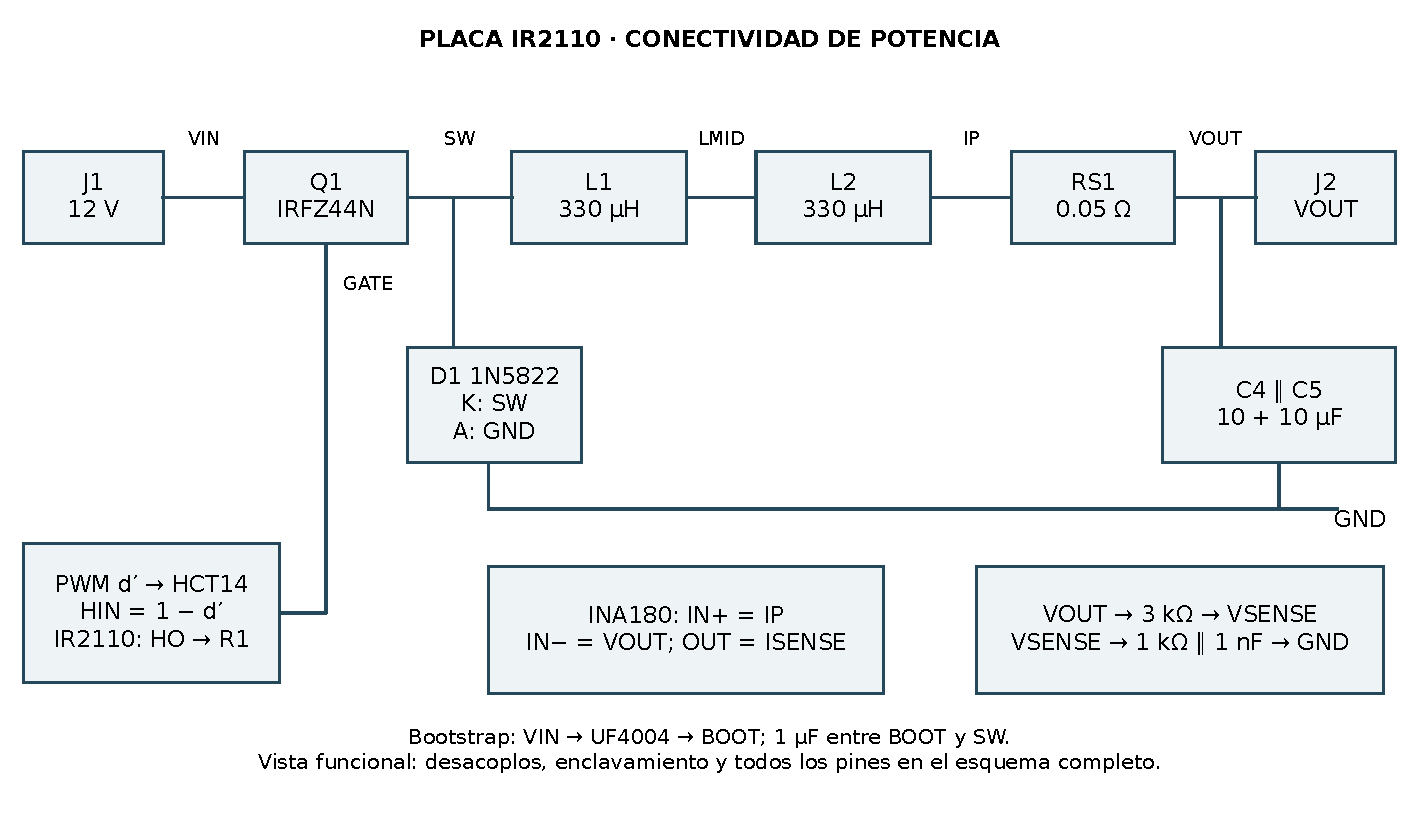
\includegraphics[width=\textwidth]{assets/power-summary.pdf}\caption{Conectividad resumida de potencia, driver y sensor de la placa IR2110. El esquema completo con todos los pines está en el anexo de hardware.}\label{fig:pcb-power}\end{figure*}
\begin{figure}[H]\centering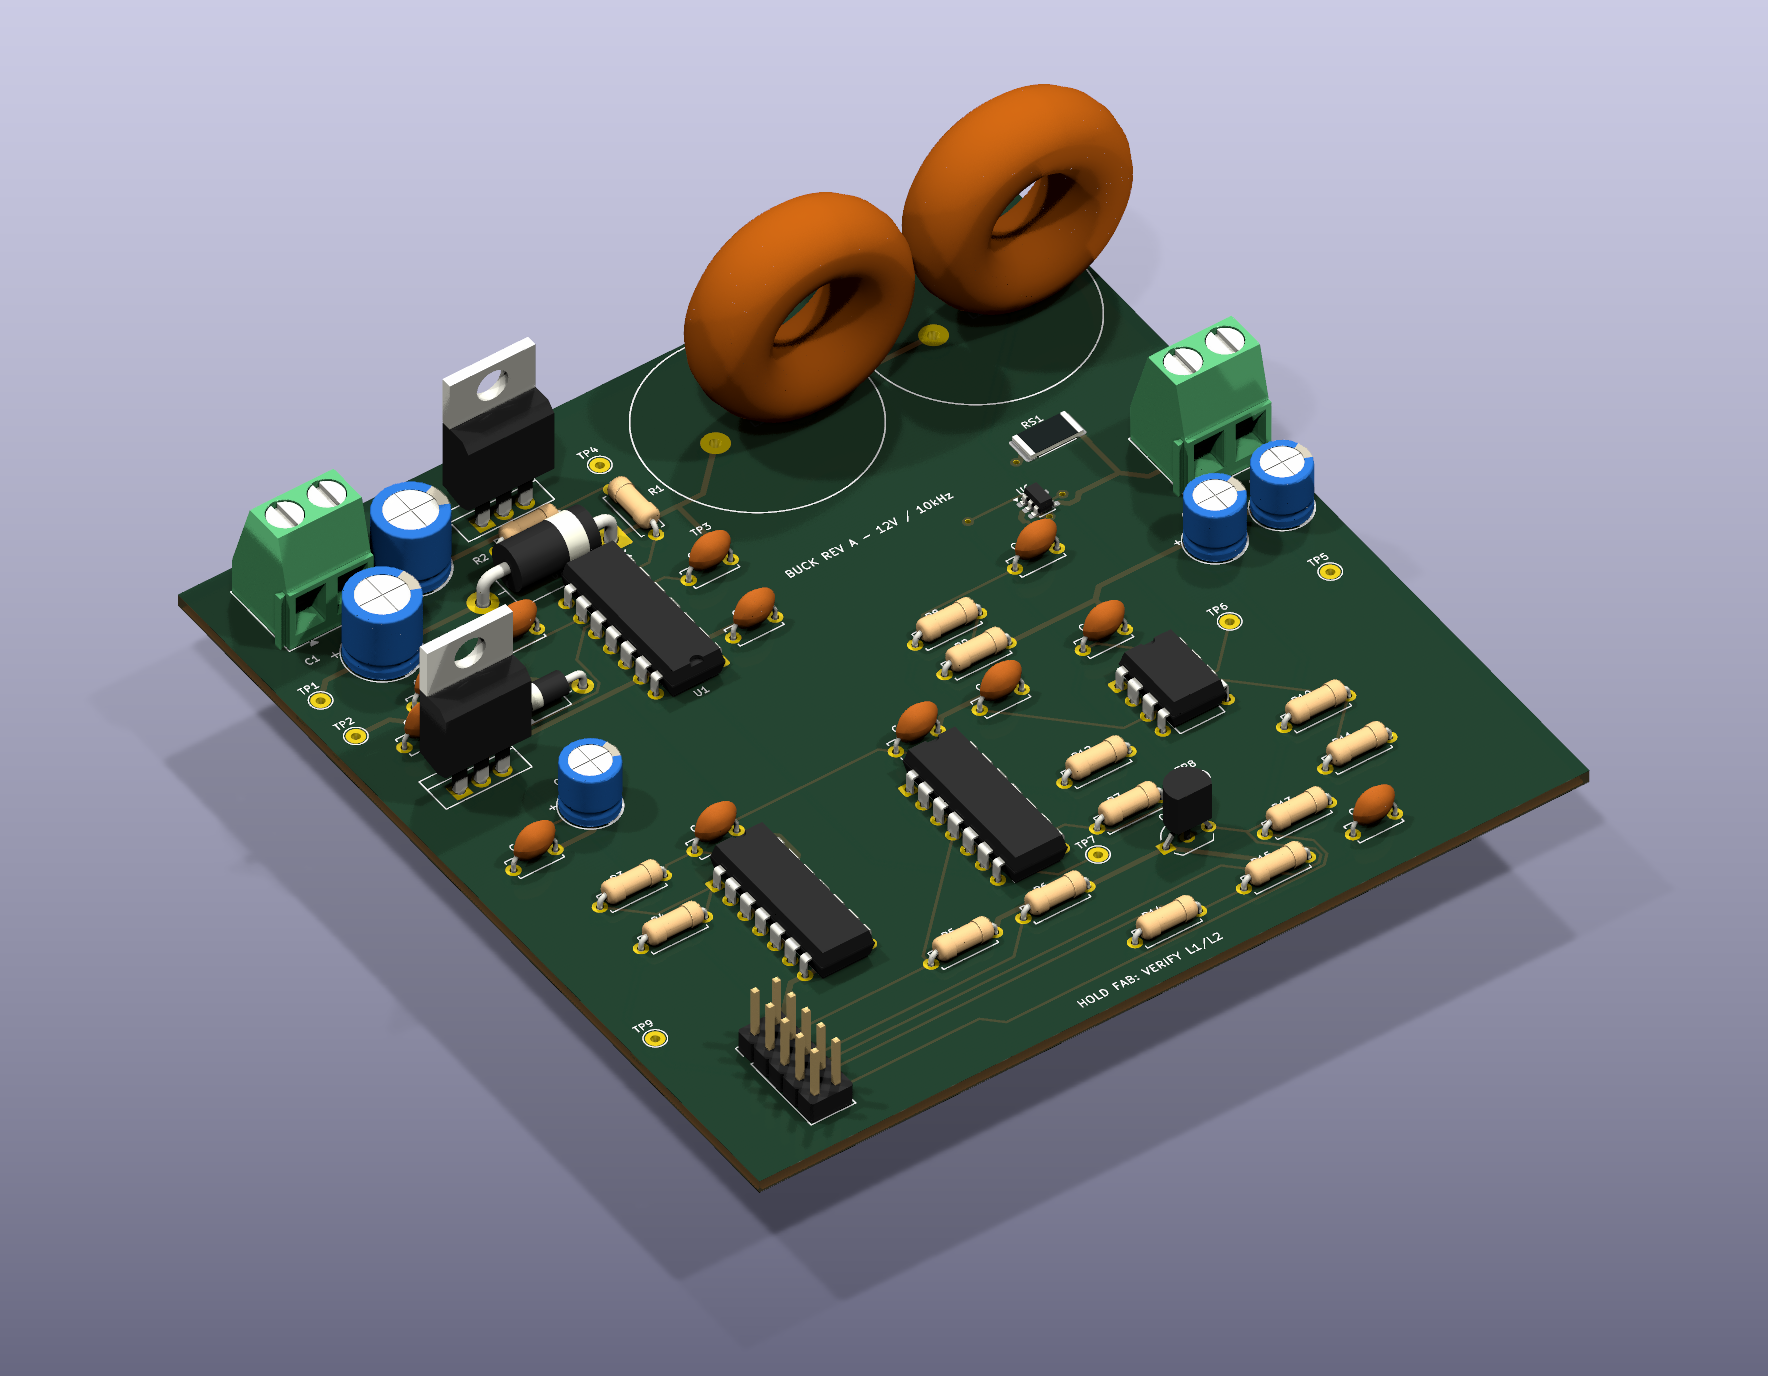
\includegraphics[width=\columnwidth]{assets/pcb-3d.png}\caption{Vista CAD isométrica; no es una fotografía. Inductores: envolvente provisional. Capacitores: geometría genérica del encapsulado, referencia comercial pendiente.}\label{fig:pcb-3d}\end{figure}
\begin{figure}[H]\centering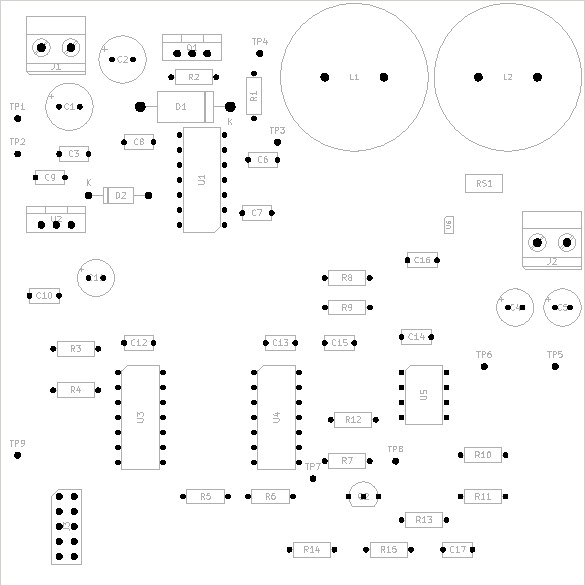
\includegraphics[width=\columnwidth]{assets/layout.pdf}\caption{Vista de componentes con referencias y conectores. Las conexiones externas se detallan en el anexo.}\label{fig:pcb-layout}\end{figure}
La fabricación permanece retenida hasta confirmar dimensiones, saturación y DCR de L1/L2, referencia y corriente de rizado de C4/C5, y verificar bootstrap, apagado y sensores en prototipo soldado. El STM32, programador y banco de carga se conectan externamente. El objetivo de presupuesto es COP 350\,000; el estimado de COP 281\,501.95 incluye asignaciones sin cotización final, dejando COP 68\,498.05 de reserva.

\section{Identificación de parámetros}
\begin{table}[H]\caption{Registro con medidor de parámetros; P = pendiente}\label{tab:measured}\centering\footnotesize\setlength{\tabcolsep}{2pt}\renewcommand{\arraystretch}{1.18}\begin{tabularx}{\columnwidth}{LYYY}\toprule
Dato & Nominal & Medido & Incert.\\\midrule
$V_{\mathrm{in}}$ (V) & 12 & P & P\\
$R$ ($\Omega$) & 6 & P & P\\
$L$ ($\mu$H) & 660 & P & P\\
$C$ ($\mu$F) & 20 & P & P\\
$r_L$ ($\Omega$) & 0.20 (sup. PCB) & P & P\\
$r_C$ ($\Omega$) & 0.15 (sup. PCB) & P & P\\
PWM (kHz) & 10 & P & P\\\bottomrule\end{tabularx}\end{table}
Registrar instrumento, identificación, calibración, frecuencia de prueba, resolución, fecha y temperatura. Medir sin energizar; comprobar ausencia de saturación del inductor bajo corriente. Conservar fotografías y datos originales.

\section{Modelo con parámetros medidos}
El subíndice $m$ denota parámetros medidos. La comparación principal actualiza la planta ideal:

\begin{equation}\label{eq:measuredplant}G_{d^{\prime},m}(s)=\frac{-V_{\mathrm{in},m}}{L_mC_ms^2+(L_m/R_m)s+1}.\end{equation}
Como contraste adicional, incluir DCR y omitir ESR conduce a:

\begin{equation}\label{eq:lossplant}\begin{aligned}G_{d^{\prime},r_L}(s)&=\frac{-V_{\mathrm{in},m}}{D_m(s)},\\D_m(s)&=L_mC_ms^2+(L_m/R_m+r_LC_m)s\\&\quad+1+r_L/R_m.\end{aligned}\end{equation}
Este segundo modelo no incorpora caídas de diodos ni driver. El analizador disponible resuelve el modelo ideal con parámetros medidos y duty registrado; no identifica automáticamente pérdidas. Inicializar con tensión y corriente previas medidas. Si falta corriente, declarar $i_L(t_i)=v_o(t_i)/R_m$ como hipótesis.

\section{Procedimiento de adquisición}
Comprobar continuidad, polaridad, PWM y apagado sin potencia. Verificar que aumentar $d^{\prime}$ reduce el tiempo ON. Energizar con fuente limitada y observar corriente y $v_{GS}$. En nodos flotantes usar medida diferencial apropiada; no conectar allí la masa de una sonda referida a tierra.

Estabilizar con $d^{\prime}=0.5$. Aplicar por separado $0.5\to0.6$ y $0.5\to0.4$, regresando al nominal entre capturas. Registrar duty y tensión simultáneamente al menos $5\,\mathrm{ms}$ antes y $20\,\mathrm{ms}$ después. Realizar tres repeticiones de cada caso.

Para rizado adquirir al menos $200\,\mathrm{kS/s}$; documentar ancho de banda y desfase de canales. Promediar periodos completos sincronizados al PWM y conservar la forma instantánea.

\section{Análisis y tablas de resultados}
Se compara la media por periodo $\bar v_c[k]$ con el modelo $v_m[k]$ interpolado en el centro de cada periodo. Para $N$ muestras:

\begin{equation}\label{eq:errors}\begin{aligned}e_k&=\bar v_c[k]-v_m[k],\\E_{\mathrm{RMS}}&=\sqrt{\frac1N\sum_{k=1}^N e_k^2},\quad E_{\max}=\max_k|e_k|.\end{aligned}\end{equation}
El error incremental resta a cada curva su propia media previa al evento, $v_{c,0}$ o $v_{m,0}$:

\begin{equation}\label{eq:incremental}e_{\Delta,k}=(\bar v_c[k]-v_{c,0})-(v_m[k]-v_{m,0}).\end{equation}
$E_{\mathrm{RMS},\Delta}$ usa la misma raíz cuadrática con $e_{\Delta,k}$. El error normalizado es $100E_{\mathrm{RMS}}/|\Delta V_{\mathrm{ideal}}|$, donde el cambio nominal tiene magnitud $1.2\,\mathrm{V}$.

\begin{table}[H]\caption{Resultados experimentales: $d^{\prime}$ $0.5\to0.6$}\label{tab:lab-up}\centering\footnotesize\setlength{\tabcolsep}{2pt}\renewcommand{\arraystretch}{1.18}\begin{tabularx}{\columnwidth}{LYY}\toprule
Magnitud & Modelo medido & Experimento\\\midrule
$v_{o,0}$; $v_{o,\infty}$ (V) & Pendiente & Pendiente\\
$M_p$ (\%); $t_s$ (ms) & Pendiente & Pendiente\\
$E_{\mathrm{RMS}}$; $E_{\max}$ (V) & --- & Pendiente\\
$E_{\mathrm{RMS},\Delta}$ (V) & --- & Pendiente\\
Rizado (V) & No incluido & Pendiente\\\bottomrule\end{tabularx}\end{table}
\begin{table}[H]\caption{Resultados experimentales: $d^{\prime}$ $0.5\to0.4$}\label{tab:lab-down}\centering\footnotesize\setlength{\tabcolsep}{2pt}\renewcommand{\arraystretch}{1.18}\begin{tabularx}{\columnwidth}{LYY}\toprule
Magnitud & Modelo medido & Experimento\\\midrule
$v_{o,0}$; $v_{o,\infty}$ (V) & Pendiente & Pendiente\\
$M_p$ (\%); $t_s$ (ms) & Pendiente & Pendiente\\
$E_{\mathrm{RMS}}$; $E_{\max}$ (V) & --- & Pendiente\\
$E_{\mathrm{RMS},\Delta}$ (V) & --- & Pendiente\\
Rizado (V) & No incluido & Pendiente\\\bottomrule\end{tabularx}\end{table}
Reportar media y dispersión de las tres repeticiones, ventanas y banda del 2\% respecto del cambio final de cada curva. La comparación absoluta evalúa exactitud; la incremental separa sesgo y dinámica. No afirmar cumplimiento de una banda menor que la incertidumbre instrumental.

\section{Discusión y criterio de cierre}
Superponer modelo nominal, modelo medido y experimento. Explicar tolerancias, pérdidas y errores instrumentales con evidencia. El cierre requiere ambas respuestas, parámetros medidos, incertidumbre, fotografías y conclusiones basadas en capturas. La validación física permanece pendiente.

\appendices\section{Archivos de análisis}\begingroup\raggedright
El CSV contiene \texttt{time\_s}, \texttt{voltage\_V}, \texttt{dprime}, \texttt{load\_ohm} y \texttt{reference\_V}. El JSON contiene \texttt{Vin}, \texttt{L\_H}, \texttt{C\_F}, \texttt{R\_ohm}, \texttt{step\_time\_s}, instrumento y fecha; \texttt{initial\_current\_A} es opcional. Ejecutar \texttt{analyze\_experiment.py} según \texttt{project/data/README.md}. Conservar calibración y archivos originales de cada repetición.

\par\endgroup
\begin{thebibliography}{9}
\bibitem{guide}J. D. Bastidas Rodríguez, ``Proyecto de Curso: Convertidor Buck con control de tensión de salida, Universidad Nacional de Colombia, mayo 2025, pp. 1--3.
\end{thebibliography}\end{document}
